\documentclass[12pt, a4paper]{article}
\setlength{\parindent}{0pt}
\usepackage[utf8]{inputenc}
\usepackage[spanish]{babel}
\usepackage{hyperref}
\usepackage{graphicx}
\usepackage{wrapfig}
\usepackage{caption}
\usepackage{subcaption}
\usepackage{multirow} 
\usepackage{ amssymb }
\usepackage{amsmath}

\begin{document} 
\title{Trabajo Práctico 2\\ Machine Learning} 
\author{Bianchi, Gabina Luz} 
\maketitle
\section*{Ejercicio A}

En este ejercicio se pide entrenar neuronas para el conjunto de datos \textit{dos elipses}, con 500 patrones en el conjunto de entrenamiento (de los cuales 400 se usan para entrenar y 100 para validar el modelo), 2000 patrones de test, 40000 épocas de entrenamiento (grabando resultados cada 400 épocas), variando los parámetros \textit{learning rate} y \textit{momentum}.

\bigskip

En la Figura 1 se presenta una tabla con los resultados promedios de error porcentual en test obtenidos en las pruebas que se realizaron. Los valores considerados para \textit{learning rate} fueron 0.1, 0.01 y 0.001, y para \textit{momentum} 0, 0.5 y 0.9. De cada combinación se hicieron 20 ejecuciones. 

\begin{figure}
    \centering
	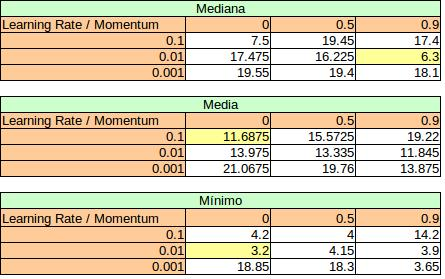
\includegraphics[scale=0.70]{tablaA}
	\caption{Resultados de error porcentual en test al entrenar neuronas para el conjunto de dato dos elipses}
\end{figure}

En este ejercicio es interesante analizar cuáles son los efectos del learning rate y del momentum. Por un lado, el learning rate indica de qué tamaño es cada paso en la trayectoria del descenso por el gradiente. Si se elige un valor muy pequeño, es factible que la búsqueda del descenso por el gradiente encuentre un mínimo local. Por el otro, el momentum tiene el efecto de mantener la dirección de la búsqueda en la misma dirección de una iteración a la siguiente. Esto podría generar que la búsqueda por el gradiente no se quede en un mínimo local cuando sin momentum sí lo haría. 

\bigskip

Para analizar esto con mayor profundidad, observaremos con detenemiento los resultados presentados en la Figura 1. \\
Un caso muy claro de estos efectos se puede apreciar en los resultados al utilizar un learning rate muy pequeño (0.001) y un momentum de 0 o 0.5. En estos dos casos se observa algo similar: la mediana, la media y el mínimo tienen valores muy altos y muy cercanos entre sí. Considerando el análisis general hecho anteriormente, es posible que al usar un paso muy pequeño en el descenso por el gradiente, la búsqueda se quede trabada en un mínimo local. Así mismo, el momentum inexistente o bajo, no permite que la búsqueda atraviece ese mínimo.\\
En la Figura 2 se pueden observar algunas gráficas de MSE en función de las épocas para ejecuciones con los valores de learning rate y momentum analizados arriba. En la Figura 2 (a) se puede ver que en ningún momento se hace algún aprendizaje, el MSE permanece constante. En la Figura 2 (b) y Figura 2 (c), se puede observar que el MSE baja fuertemente a partir de alguna época. Sin embargo, posiblemente allí la búsqueda del descenso por el gradiente haya caído en un mínimo local.


\begin{figure}
    \centering

    \begin{subfigure}[b]{0.45\textwidth}
        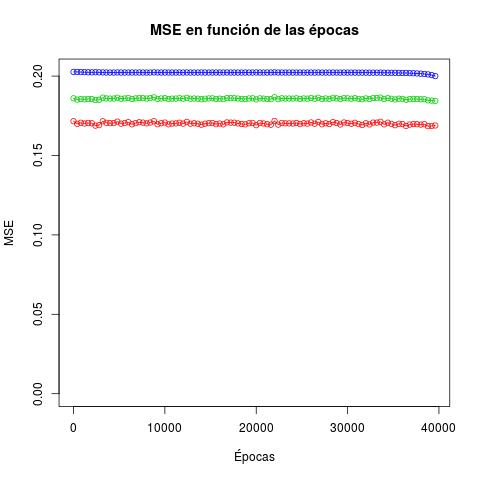
\includegraphics[width=\textwidth]{mse13d}
        \caption{Momentum = 0}
        %\label{fig:tiger}
    \end{subfigure}
      ~ %add desired spacing between images, e. g. ~, \quad, \qquad, \hfill etc. 
      %(or a blank line to force the subfigure onto a new line)
    \begin{subfigure}[b]{0.45\textwidth}
        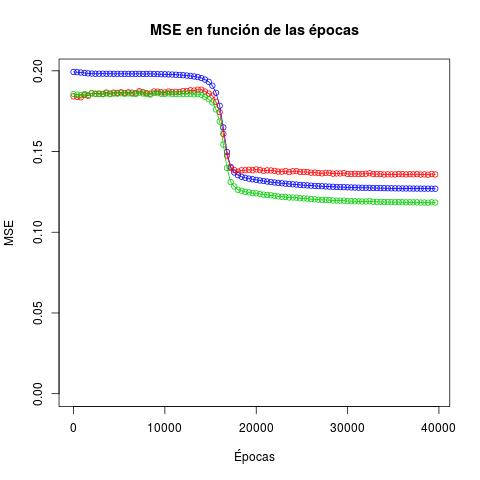
\includegraphics[width=\textwidth]{mse13c}
        \caption{Momentum = 0}
        %\label{fig:gull}
    \end{subfigure}
    ~ %add desired spacing between images, e. g. ~, \quad, \qquad, \hfill etc. 
      %(or a blank line to force the subfigure onto a new line)
    \begin{subfigure}[b]{0.45\textwidth}
        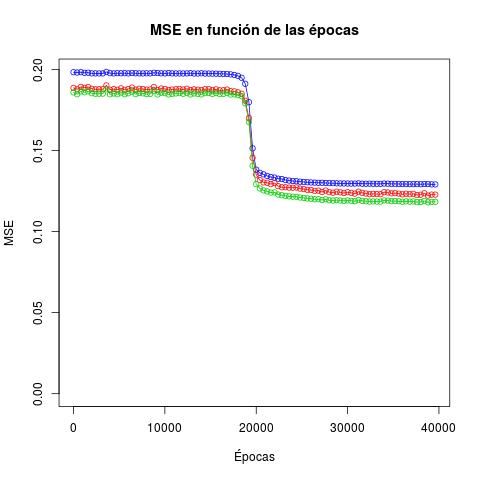
\includegraphics[width=\textwidth]{mse23}
        \caption{Momentum = 0.5}
        %\label{fig:tiger}
    \end{subfigure}
    \caption{MSE en función de las épocas utilizando un learning rate de 0.001. Las curvas azules representan el MSE de entrenamiento, las rojas de validación y las verdes de test.}
\end{figure}

\bigskip

Al analizar el resultado para igual learning rate pero momentum de 0.9, se puede observar que la mediana sigue tomando un valor muy alto, pero la media y sobre todo el mínimo disminuyen. Estos valores (quizás) nos indican que en algunos casos (pero no en todos) el descenso por el gradiente logra atravezar algunos mínimos locales (quizás para trabarse en un nuevo mínimo local, pero menor). Este hecho lo podemos atribuír al momentum mayor, como se analizó antes. \\
En la Figura 3 se graficó nuevamente el MSE en función de las épocas para la combinación de valores analizada. En la Figura 3 (a) se está en un caso similar a los anteriores: el MSE es constante, disminuye fuertemente y luego permanece constante nuevamente. En la Figura 3 (b) posiblemente se esté observando un caso en el cual se logra atravezar un mínimo local, y por lo tanto, luego del primer descenso brusco, el MSE sigue disminyendo.


\begin{figure}
    \centering

    \begin{subfigure}[b]{0.45\textwidth}
        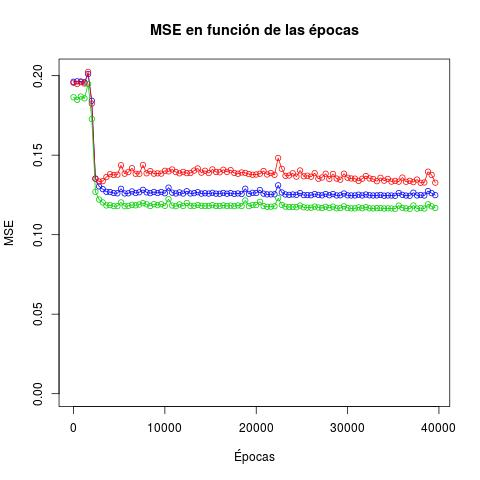
\includegraphics[width=\textwidth]{mse33}
        \caption{Momentum = 0.9}
        %\label{fig:tiger}
    \end{subfigure}
      ~ %add desired spacing between images, e. g. ~, \quad, \qquad, \hfill etc. 
      %(or a blank line to force the subfigure onto a new line)
    \begin{subfigure}[b]{0.45\textwidth}
        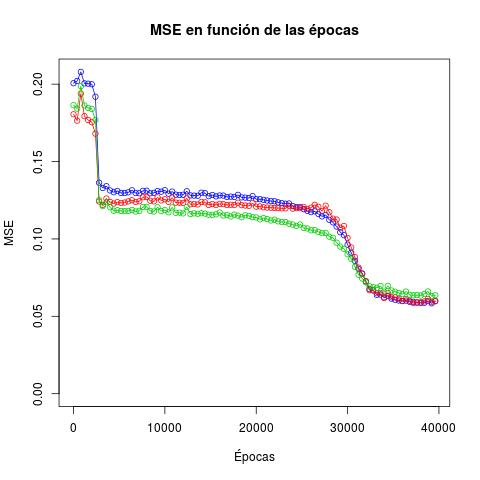
\includegraphics[width=\textwidth]{mse33e}
        \caption{Momentum = 0.9}
        %\label{fig:gull}
    \end{subfigure}
    \caption{MSE en función de las épocas utilizando un learning rate de 0.001. Las curvas azules representan el MSE de entrenamiento, las rojas de validación y las verdes de test.}
\end{figure}

\bigskip

Los casos en los cuales las redes se entrenaron con learning rate igual 0.01 y momentum 0 o 0.5 son similares entre sí. Ambos resultados presentan medianas altas, promedios más bajos y mínimos buenos. Estos valores nos indican que nuevamente hay ejecuciones en las cuales la búsqueda de descenso por el gradiente encuentra mínimos locales, y otras en las que lo logra atravezar al menos algunos de ellos. \\
Si consideramos la ejecución que utiliza momentum 0, el hecho de que logre sortear algunos mínimos locales se puede atribuír a que el paso no es tan pequeño. Es decir, quizás al dar un paso mayor salta los \textquotedblleft pozos\textquotedblright pequeños. Para el caso en que se utiliza momentum de 0.5, los resultados se puede atribuír no únicamente al paso mayor, si no también al valor del momentum.\\
En la Figura 4 se graficó el MSE en función de las épocas. En la Figura 4 (a) se puede observar un caso en el cual posiblemente la búsqueda se haya estancado en un mínimo local, mientras que en la Figura 4 (b) se observa que el MSE sigue disminuyendo luego de la caída abrupta, para un momentum 0. La Figura 4 (c) y es análoga a la Figura 4 (a), pero el momentum utilizado es de 0.5. En la figura 4 (d) se observa que el MSE vuelve a estancarse luego de la segunda caída abrupta, pero en un valor menor. Posiblemente haya encontrado un nuevo mínimo local pero mejor.



\begin{figure}
    \centering

    \begin{subfigure}[b]{0.45\textwidth}
        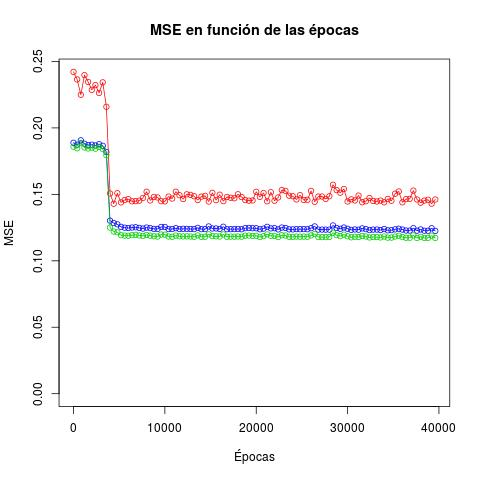
\includegraphics[width=\textwidth]{mse12}
        \caption{Momentum = 0}
        %\label{fig:tiger}
    \end{subfigure}
      ~ %add desired spacing between images, e. g. ~, \quad, \qquad, \hfill etc. 
      %(or a blank line to force the subfigure onto a new line)
    \begin{subfigure}[b]{0.45\textwidth}
        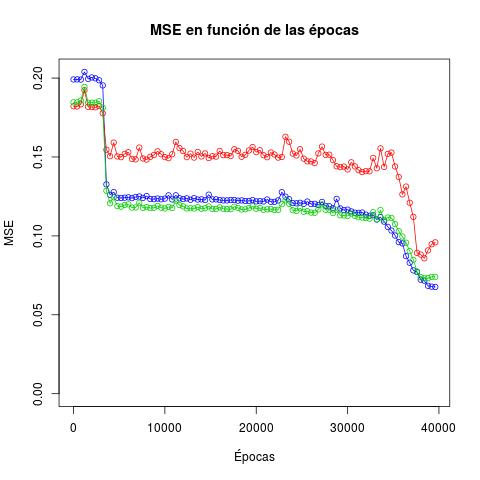
\includegraphics[width=\textwidth]{mse12e}
        \caption{Momentum = 0}
        %\label{fig:gull}
    \end{subfigure}
    ~ %add desired spacing between images, e. g. ~, \quad, \qquad, \hfill etc. 
      %(or a blank line to force the subfigure onto a new line)
    \begin{subfigure}[b]{0.45\textwidth}
        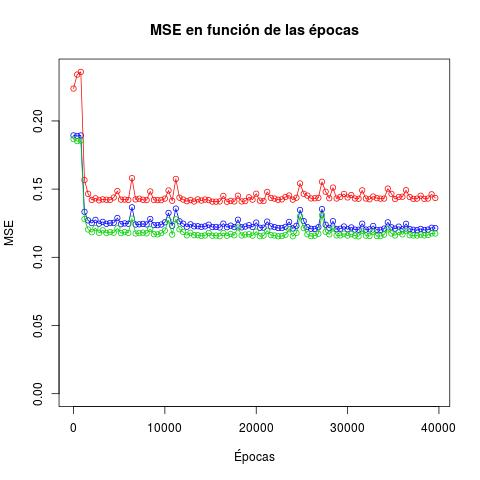
\includegraphics[width=\textwidth]{mse22}
        \caption{Momentum = 0.5}
        %\label{fig:tiger}
    \end{subfigure}
    ~ %add desired spacing between images, e. g. ~, \quad, \qquad, \hfill etc. 
      %(or a blank line to force the subfigure onto a new line)
    \begin{subfigure}[b]{0.45\textwidth}
        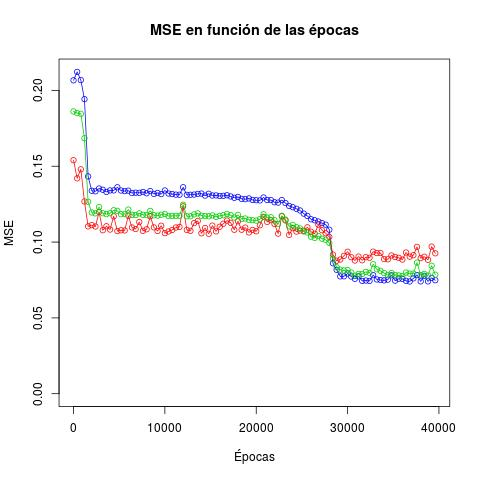
\includegraphics[width=\textwidth]{mse22b}
        \caption{Momentum = 0.5}
        %\label{fig:tiger}
    \end{subfigure}    
    \caption{MSE en función de las épocas utilizando un learning rate de 0.01. Las curvas azules representan el MSE de entrenamiento, las rojas de validación y las verdes de test.}
\end{figure}

\bigskip

El resultado de ejecuciones utilizando un learning rate 0.01 y un momentum de 0.9 es similar a los casos analizados anteriormente, exceptuando su mediana llamativamente pequeña (de hecho, la menor de todas las conseguidas). Estos valores nos indican que la mitad de las ejecuciones obtuvo un error porcentual en test menor o igual a 6.3. La otra mitad posiblemente haya tenido valores altos, por eso levantan tanto el promedio. El hecho de que muchas ejecuciones hayan logrado sortear mínimos locales se le puede atribuír justamente al momentum alto. \\
Nuevamente en la Figura 5 se graficó MSE en función de las épocas para distintas ejecuciones. En la Figura 5 (a) podría estarse en un caso mayor a la mediana, mientras que en la Figura 5 (b), en un caso menor a la misma.


\begin{figure}
    \centering

    \begin{subfigure}[b]{0.45\textwidth}
        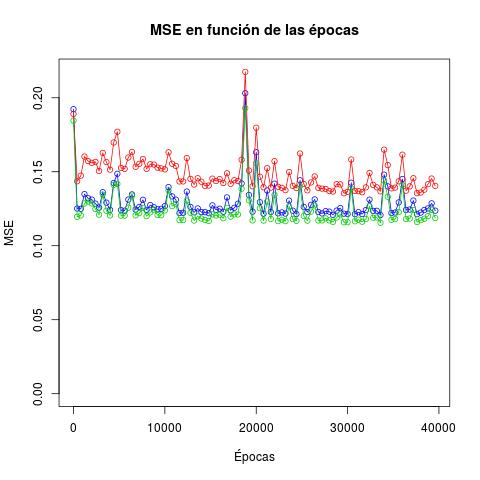
\includegraphics[width=\textwidth]{mse32}
        \caption{Momentum = 0.9}
        %\label{fig:tiger}
    \end{subfigure}
      ~ %add desired spacing between images, e. g. ~, \quad, \qquad, \hfill etc. 
      %(or a blank line to force the subfigure onto a new line)
    \begin{subfigure}[b]{0.45\textwidth}
        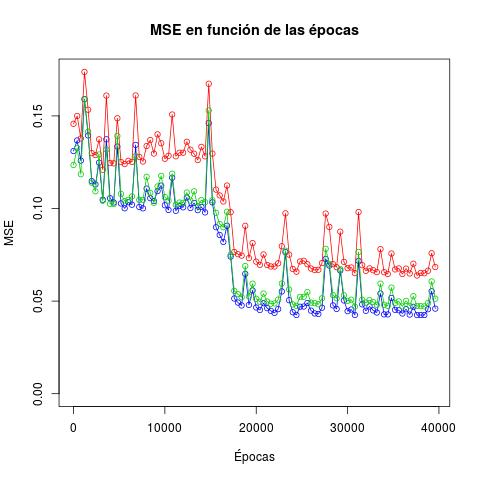
\includegraphics[width=\textwidth]{mse32c}
        \caption{Momentum = 0.9}
        %\label{fig:gull}
    \end{subfigure}

    \caption{MSE en función de las épocas utilizando un learning rate de 0.01. Las curvas azules representan el MSE de entrenamiento, las rojas de validación y las verdes de test.}
\end{figure}

\bigskip

Por último, quedan analizar las ejecuciones en las que se utilizó un learning rate de 0.1. Por un lado se debe tener en cuenta que al ser mayor el paso con que se \textquotedblleft avanza\textquotedblright en la búsqueda del descenso por el gradiente, la función de error se verá más discontinua. Es decir, cambiará más de una iteración a la otra. Esta tendencia aumenta cunado el momentum utilizado es mayor. Este fenómeno ya se podía observar en la última gráfica analizada, la Figura 5, en donde se utilizó un learning rate de 0.01 y un momentum de 0.5.\\
La ejecución en la cual no se utilizó momentum, presenta resultados similares a los anteriores. Existen casos en donde la búsqueda del descenso por el gradiente pareciera rápidamente quedarse atascada en mínimos locales, y otros en donde el MSE logra disminuír más. Esto se puede apreciar en la Figura 6 (a) y la Figura 6 (b), respectivamente.\\
El caso en el cual se utilizó learning rate de 0.1 y momentum de 0.5, presenta un buen mínimo pero una mediana y una media alta. En la Figura 7 (a) se puede observar la gráfica de MSE en función de las épocas, que posiblemente represente a la mayoría de las ejecuciones de esta clase. Allí se puede observar que los puntos son muy distintos de una iteración a la otra, pero que la tendencia del MSE es mantenerse constante.\\
El análisis hecho recientemente se acentúa si se observa la Figura 7 (b), en la cual se utilizó un momentum de 0.9. Allí el MSE es más alto, y los puntos más distantes entre sí. A su vez, si se mira la tabla, el mínimo que se presenta es considerablemente alto.

\bigskip
Como conclusión de este análisis se puede decir que en general, utilizar un learning rate y un momentum muy altos, o muy bajos, no presenta buenos resultados. En estas ejecuciones las redes neuronales tienden a caer en mínimos locales muy rápidamente o a no hacer ninguna clase de aprendizaje, manteniendo las curvas de MSE constantes. Por el contrario, utilizar valores de learning rate y momentum intermedios, o utilizar momentum grande y learning rate pequeño o viceversa, presenta mejores resultados.\\
A su vez, otra cuestión a resaltar es que los mínimos puede ser engañosos. Existen casos en los cuales una cierta combinación de learning rate y momentum obtiene un mínimo muy bueno, pero sin embargo, su media y su mediana son considerablemente altas. Esto quiere decir que en general, las redes no están teniendo buenos rendimientos, pero ocasionalmente sí lo pueden tener.


\begin{figure}
    \centering

    \begin{subfigure}[b]{0.45\textwidth}
        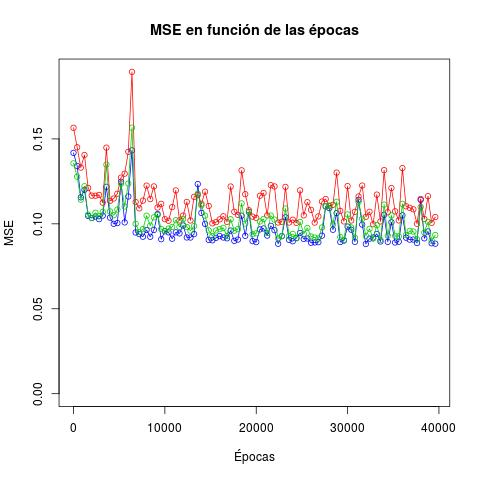
\includegraphics[width=\textwidth]{mse11}
        \caption{Momentum = 0}
        %\label{fig:tiger}
    \end{subfigure}
      ~ %add desired spacing between images, e. g. ~, \quad, \qquad, \hfill etc. 
      %(or a blank line to force the subfigure onto a new line)
    \begin{subfigure}[b]{0.45\textwidth}
        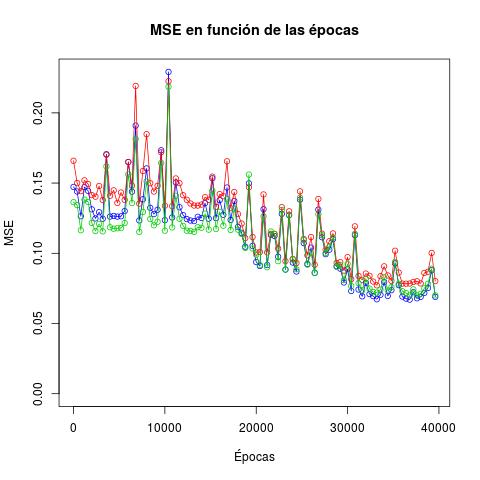
\includegraphics[width=\textwidth]{mse11d}
        \caption{Momentum = 0}
        %\label{fig:gull}
    \end{subfigure}

    \caption{MSE en función de las épocas utilizando un learning rate de 0.1. Las curvas azules representan el MSE de entrenamiento, las rojas de validación y las verdes de test.}
\end{figure}

\begin{figure}
    \centering

    \begin{subfigure}[b]{0.45\textwidth}
        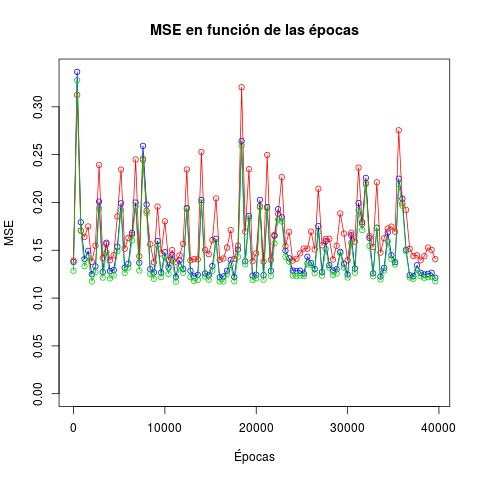
\includegraphics[width=\textwidth]{mse21d}
        \caption{Momentum = 0.5}
        %\label{fig:tiger}
    \end{subfigure}
      ~ %add desired spacing between images, e. g. ~, \quad, \qquad, \hfill etc. 
      %(or a blank line to force the subfigure onto a new line)
    \begin{subfigure}[b]{0.45\textwidth}
        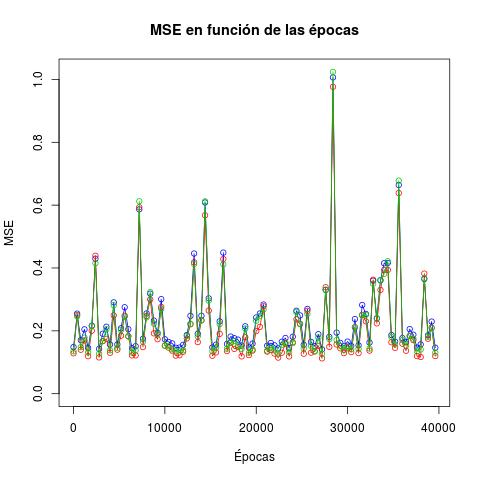
\includegraphics[width=\textwidth]{mse31}
        \caption{Momentum = 0.9}
        %\label{fig:gull}
    \end{subfigure}

    \caption{MSE en función de las épocas utilizando un learning rate de 0.1. Las curvas azules representan el MSE de entrenamiento, las rojas de validación y las verdes de test.}
\end{figure}
 

\section*{Ejercicio B}

En este ejercicio se pide entrenar redes neuronales con el conjunto de datos de las espirales anidadas, con learning rate de 0.01, momentum de 0.5, 1600 datos para ajustar los modelos, 400 para validar, 2000 para testear, 40000 épocas de entrenamiento (grabando cada 400), variando el número de neuronas en la capa intermedia entre 2, 5, 10, 20 y 40. 

\bigskip
 
Por lo tanto, en este caso es interesante analizar cómo influye la arquitectura de la red neuronal en sus predicciones. En la Figura 8 se muestra un ejemplo de la estructura de la red neuronal con 2 neuronas en la capa intermedia. 
 

 
\begin{figure}
    \centering
	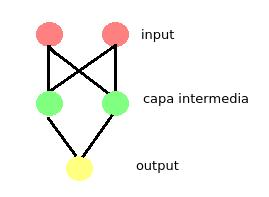
\includegraphics[scale=0.65]{neurona}
	\caption{Ejemplo de la arquitectura de red neuronal utilizada, con 2 neuronas en la capa intermedia.}
\end{figure} 
 
\bigskip  
 
El objetivo de las neuronas ocultas es capturar características de los datos de entrenamiento que no están explícitas en las entradas. De alguna manera, la capa intemedia captura las propiedades más importantes de los inputs, de modo de acercarse a la función objetivo.\\ 
Al aumentar el número de neuronas ocultas, aumenta también la cantidad de pesos. De esta manera, la superficie de error que considera el algoritmo backpropagation comienza a ser más compleja. \footnote{Recordemos que la función \textit{E} utilizada por el algoritmo backpropagation toma como argumento el vector $\vec{w}$, el cual es el vector que contiene todos los pesos de la red. Por lo tanto, al haber más cantidad de pesos, la función comienza a tener más dimensiones.} En este sentido, puede pensarse que mientras más dimensiones tenga la superficie de error, menos probable es que la búsqueda del descenso por el gradiente encuentre un mínimo local. Esto es debido a que cada dimensión puede ser una \textquotedblleft ruta de escape \textquotedblright. Es decir, para caer en un mínimo local, todas las dimensiones deben caer en un mínimo local.

\bigskip

De esta manera, es esperable que al aumentar el número de neuronas en la capa intermedia, disminuya el error en las predicciones (aunque se sabe, el tiempo de ejecución aumenta considerablemente). En la Figura 9 se presenta una tabla con los resultados de error porcentual en test obtenidos, y en la Figura 10, las predicciones en función de la cantidad de neuronas ocultas utilizadas. Dichas figuras refuerzan la idea presentada anteriormente.


\begin{figure}
    \centering
	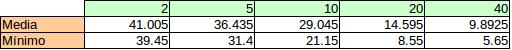
\includegraphics[scale=1]{tablaB}
	\caption{Resultados de error porcentual en test al entrenar neuronas para el conjunto de dato espirales anidadas según la cantidad de neuronas utilizadas en la capa intermedia.}
\end{figure}
 
\bigskip


\begin{figure}
    \centering

    \begin{subfigure}[b]{0.4\textwidth}
        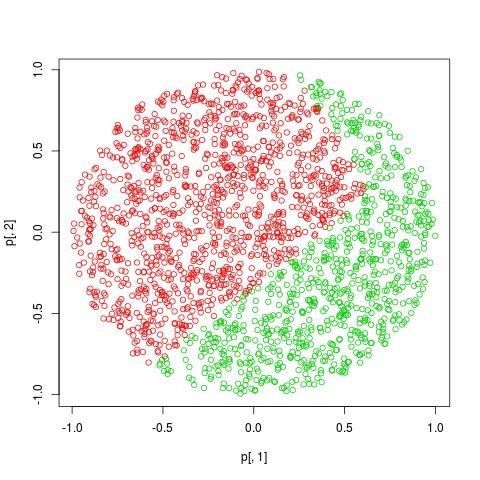
\includegraphics[width=\textwidth]{prediccion1}
        \caption{2 neuronas}
        %\label{fig:tiger}
    \end{subfigure}
      ~ %add desired spacing between images, e. g. ~, \quad, \qquad, \hfill etc. 
      %(or a blank line to force the subfigure onto a new line)
    \begin{subfigure}[b]{0.4\textwidth}
        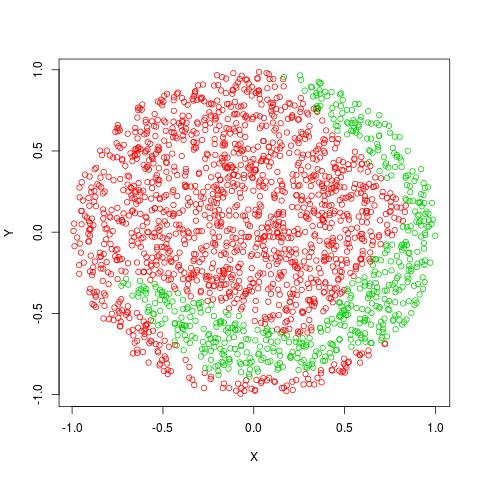
\includegraphics[width=\textwidth]{prediccion2}
        \caption{5 neuronas}
        %\label{fig:gull}
    \end{subfigure}
    ~ %add desired spacing between images, e. g. ~, \quad, \qquad, \hfill etc. 
      %(or a blank line to force the subfigure onto a new line)
    \begin{subfigure}[b]{0.4\textwidth}
        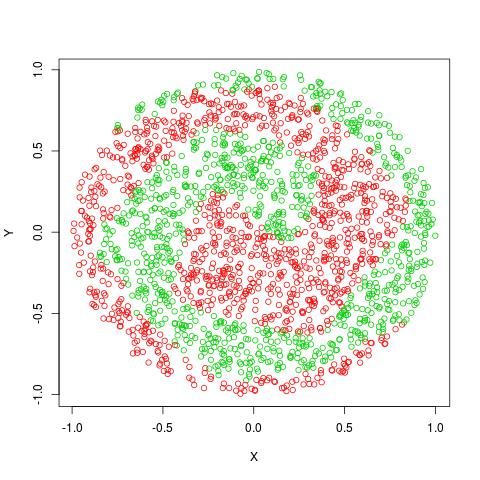
\includegraphics[width=\textwidth]{prediccion3}
        \caption{10 neuronas}
        %\label{fig:tiger}
    \end{subfigure}
    
      ~ %add desired spacing between images, e. g. ~, \quad, \qquad, \hfill etc. 
      %(or a blank line to force the subfigure onto a new line)
    \begin{subfigure}[b]{0.4\textwidth}
        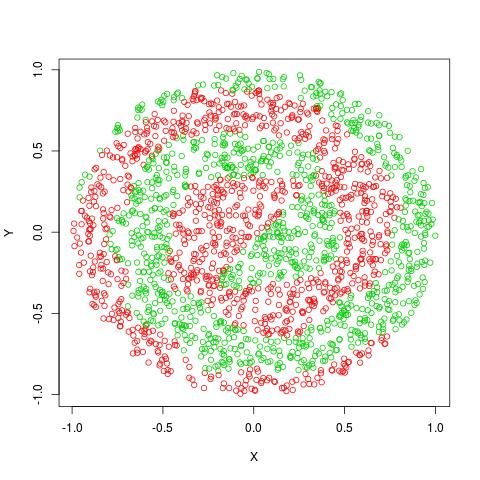
\includegraphics[width=\textwidth]{prediccion4}
        \caption{20 neuronas}
        %\label{fig:gull}
    \end{subfigure}
    ~ %add desired spacing between images, e. g. ~, \quad, \qquad, \hfill etc. 
      %(or a blank line to force the subfigure onto a new line)
    \begin{subfigure}[b]{0.4\textwidth}
        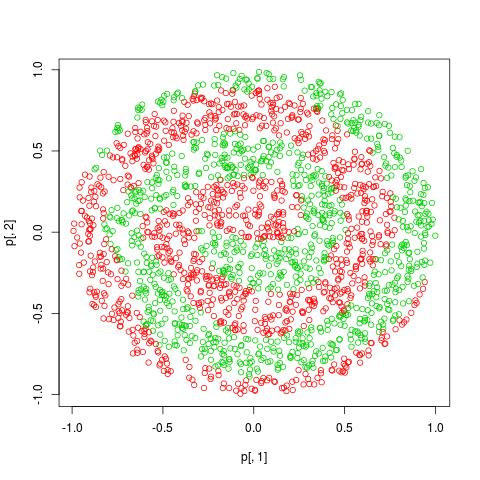
\includegraphics[width=\textwidth]{prediccion5}
        \caption{40 neuronas}
        %\label{fig:tiger}
    \end{subfigure}
        
    \caption{Predicciones del conjunto de datos de las espirales anidadas, según la cantidad de neuronas en la capa intermedia.}
\end{figure}

\newpage

\section*{Ejercicio C}

En este ejercicio se pide entrenar redes neuronales con el conjunto de datos ikeda (5 datos de entrada, 1 de salida), variando la cantidad de datos de entrenamiento y de validación. Las variaciones analizadas son: 190, 150 y 100 datos de entranamiento y 10, 50 y 100 datos de validación, respectivamente. Es decir, relaciones 95\%-5\%, 75\%-25\% y 50\%-50\%.

\bigskip

Para hacer este análisis es importante tener en cuenta que la cantidad de puntos de entrenamiento utilizados no es alta considerando que la red neuronal tiene 5 dimensiones de las cuales aprender. Si bien tener mayor número de dimensiones es tener más información, en la práctica suele ser difícil aprender correctamente en estos casos. \\
Por lo tanto, es esperable que la cantidad de puntos de entrenamiento no le permita a la red neuronal aprender las verdaderas reglas existentes entre las entradas y las salidas. Posiblemente, la red esté aprendiendo de relaciones particulares de los puntos de entrenamiento dados.
 
 \bigskip
 
En la Figura 11 se grafica el MSE en función de la cantidad de épocas cuando se entrenan las neuronas con 190 puntos de entrenamiento y 10 de validación. En los tres casos, la tendencia del MSE de test y entrenamiento es disminuír. Por lo cual se puede suponer que la red está aprendiendo correctamente. Si analizamos la curva de validación, vemos que en los tres casos tiene diferentes tendencias: en una gráfica se encuentre entre el medio de test y entrenamiento, en otra por encima de los dos, y en la tercera por debajo. A su vez, se observa que esta curva tiene muchos saltos. Todo esto se puede atribuír a que la cantidad de puntos de validación es demasiado pequeño como para estar representando algo con sentido. Es decir, el conjunto de validación utilizado no es representativo de lo que pasa con los puntos realmente.
 
 
 \begin{figure}
    \centering

    \begin{subfigure}[b]{0.45\textwidth}
        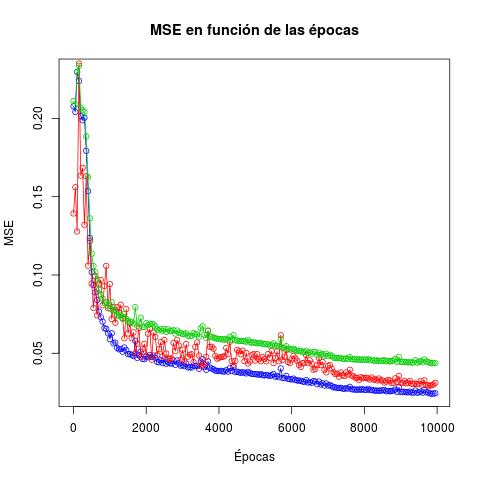
\includegraphics[width=\textwidth]{mse1b}
        %\label{fig:tiger}
    \end{subfigure}
      ~ %add desired spacing between images, e. g. ~, \quad, \qquad, \hfill etc. 
      %(or a blank line to force the subfigure onto a new line)
    \begin{subfigure}[b]{0.45\textwidth}
        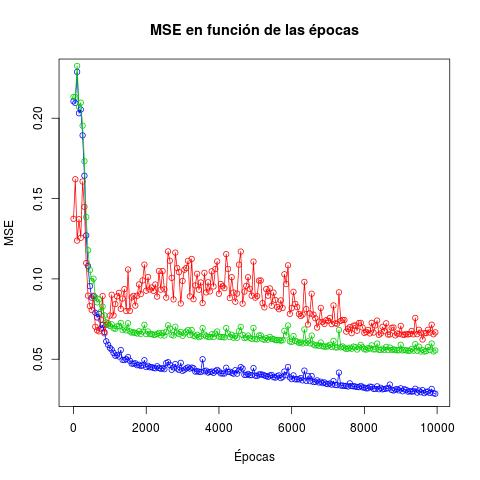
\includegraphics[width=\textwidth]{mse1c}
        %\label{fig:gull}
    \end{subfigure}
      ~ %add desired spacing between images, e. g. ~, \quad, \qquad, \hfill etc. 
      %(or a blank line to force the subfigure onto a new line)
    \begin{subfigure}[b]{0.45\textwidth}
        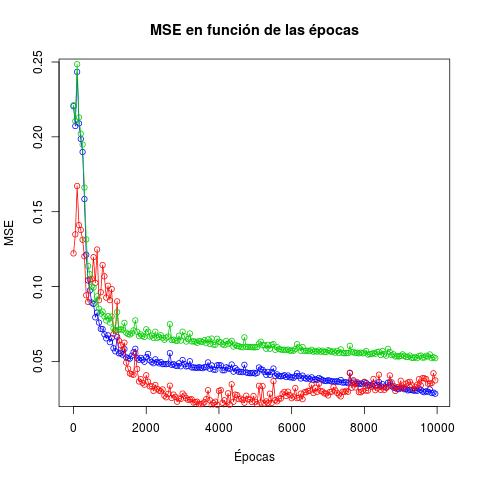
\includegraphics[width=\textwidth]{mse1d}
        %\label{fig:gull}
    \end{subfigure}    
    \caption{MSE en función de las épocas utilizando 190 puntos de entrenamiento y 10 de validación. Las curvas azules representan el MSE de entrenamiento, las rojas de validación y las verdes de test.}
\end{figure}

\bigskip
 
En la Figura 12 se grafica el MSE en función del número de épocas para las ejecuciones de la red neuronal entrenada con 150 puntos de entrenamiento y 50 de validación. En esta figura, se empieza a notar la tendencia del error en test y en validación de crecer, mientas que el error de entrenamiento sigue bajando. Es decir, comienza a apreciarse el sobreajuste. Posiblemente, la cantidad de puntos de entrenamiento ya no sea suficiente como para que la red neuronal aprenda correctamente las reglas naturales de éstos. A su vez, aún se observa que la curva de validación tiene saltos, debido a que el número de puntos de validación todavía no es lo suficientemente alto. Sin embargo, se puede notar que la curva roja es un buen indicador del sobreajuste, ya que ésta comienza a crecer junto con la curva de test. Si se eligieran los pesos correspondientes al menor MSE en validación, se obtendría el mejor resultado posible (en el test utilizado) para el aprendizaje de esta red neuronal.
 
\begin{figure}
    \centering
	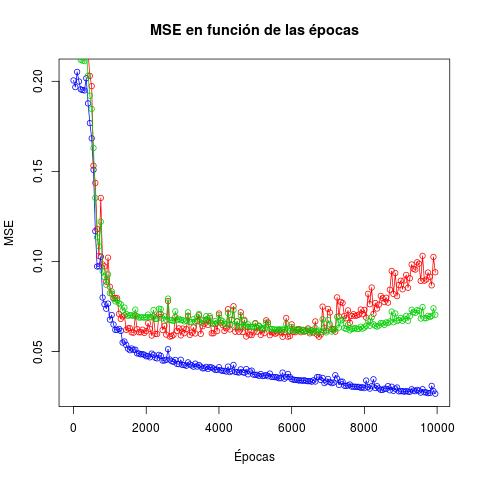
\includegraphics[scale=0.45]{mse2e}
	\caption{MSE en función de las épocas utilizando 150 puntos de entrenamiento y 50 de validación. Las curvas azules representan el MSE de entrenamiento, las rojas de validación y las verdes de test.}
\end{figure} 


\bigskip

Por último, en la Figura 13 se grafica el MSE utilizando 100 puntos de entrenamiento y 100 de validación. Allí se puede observar que la curva roja ya no presenta grandes saltos, posiblemente porque ya se está utilizando una cantidad mayor de puntos. En la Figura 13 (a) se puede observar que la curva azul tiene una tendencia a disminuír más fuertemente que en la Figura 12. Así mismo, la curva de test, a aumentar. Esto posiblemente se deba a que el conjunto de puntos de entrenamiento es más pequeño. No obstante, se puede notar que nuevamente la curva de validación es un buen indicador de sobreajuste: comienza a crecer junto con la curva de test.\\
Respecto a la Figura 13 (b), se puede decir que ese caso sirve como ejemplo de que la curva de validación puede tener disminuciones luego de un crecimiento. Es decir, en la gráfica se observa que luego del primer ascenso fuerte de la curva roja, ésta comienza a bajar. Por lo tanto, podría llegar a ser una idea no conveniente quedarse con los pesos calculados justo antes de que la curva de validación comience a crecer. Independientemente de aquello, se obserca que aún para este caso, la curva roja es un buen indicador de sobreajuste.

 \begin{figure}
    \centering

    \begin{subfigure}[b]{0.45\textwidth}
        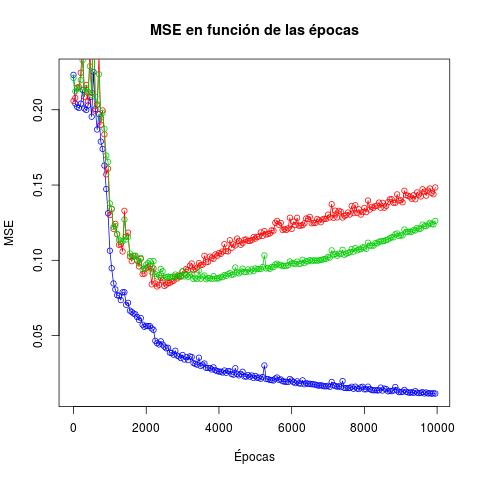
\includegraphics[width=\textwidth]{mse3b}
        %\label{fig:tiger}
    \end{subfigure}
      ~ %add desired spacing between images, e. g. ~, \quad, \qquad, \hfill etc. 
      %(or a blank line to force the subfigure onto a new line)
    \begin{subfigure}[b]{0.45\textwidth}
        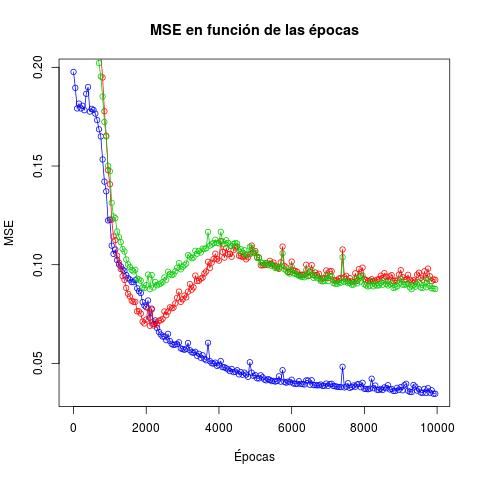
\includegraphics[width=\textwidth]{mse3c}
        %\label{fig:gull}
    \end{subfigure}
    \caption{MSE en función de las épocas utilizando 100 puntos de entrenamiento y 10 de validación. Las curvas azules representan el MSE de entrenamiento, las rojas de validación y las verdes de test.}
\end{figure}

 \bigskip
 
Como conclusión de este ejercicio, se puede decir que las curvas de validación son un buen método para calcular cuándo está comenzando a sobreajustar la red neuronal. Sin embargo, es necesario tener una cantidad de puntos medianamente alta para que la curva sea significativa. 

\section*{Ejercicio D}

En este ejercicio se pide implementar el algoritmo de regularización \textit{weight-decay}. En lugar de utilizar un conjunto distinto de datos para validación, se agrega a la función de error un término de penalización a los pesos con valor absoluto grande. Esta nueva versión de backpropagation introduce una constante $\gamma$, siendo el término de penalización igual a $\gamma \sum_{i,j}^{} w_{j,i}^2  $ . Se considera justamente una penalización porque mientras mayor magnitud tengan los pesos, dicho término crecerá, y por lo tanto el error para esos pesos tendrá una suma positiva extra. Esta técnica intenta mantener los pesos con magnitudes cercanas a cero de modo de reducir el riesgo de sobreajuste.

\bigskip

Para implementar dicho algoritmo se agregó al archivo de configuración el valor de la constante $\gamma$, se utilizó una nueva variable \textit{penalty}, la cual contiene el término de penalización para cada iteración, y se modificó la regla de actualización multiplicando cada peso por (1-2$\gamma \eta$). Esta modificación es equivalente a utilizar la nueva versión de la función error que sí posee el término de penalización.

\bigskip

Este nuevo método de regularización se aplicó al conjunto de datos sunspots, variando el valor de $\gamma$. Se consideraron valores $10^{-i}$, con $i = 0,1,...,8$.\\
Observando los resultados obtenidos se puede suponer que valores muy pequeños de $\gamma$ producen sobreajuste. Un ejemplo de la gráfica de MSE de test y entrenamiento se puede observar en la Figura 14 (a), para un valor de $\gamma = 10^{-8}$. En este caso una hipótesis posible es que al tomar el término de penalización valores tan pequeños, el algoritmo de regularización no es efectivo. Los valores que toma el término de penalización se pueden observar en la Figura 14 (b). \\
Si consideramos el caso en el cual se elegió $\gamma = 10^{-5}$, se puede observar en la Figura 15 que los valores del término de penalización son lo suficientemente grandes como para evitar el sobreajuste, y a su vez, permiten que la red neuronal aprenda. Esto se puede apreciar en el descenso que presentan las curvas de MSE de test y entrenamiento. A su vez se puede notar que, aproximadamente, a partir de la época 23000 los MSE comienzan a permanecer constantes, al mismo tiempo que el término de penalización deja de crecer.\\
Para los experimentos en los cuales se utilizaron los valores mayores de $\gamma$, se puede apreciar que, tanto las curvas de MSE como las de valor del término de penalización en función de las épocas, son muy discontinuas. A su vez, según el comportamiento del MSE, las redes neuronales parecen no estar haciendo aprendizaje, y el error es considerablemente mayor que para valores de $\gamma$ más pequeños.


 \begin{figure}
    \centering

    \begin{subfigure}[b]{0.45\textwidth}
        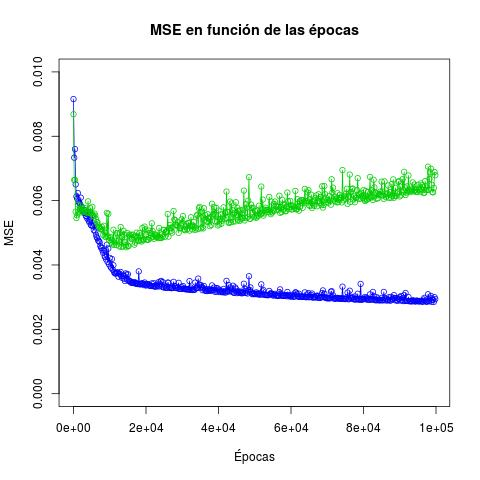
\includegraphics[width=\textwidth]{ejercicioD1}
        %\label{fig:tiger}
		\caption{MSE en test y entrenamiento en función de las épocas.}
    \end{subfigure}
      ~ %add desired spacing between images, e. g. ~, \quad, \qquad, \hfill etc. 
      %(or a blank line to force the subfigure onto a new line)
    \begin{subfigure}[b]{0.45\textwidth}
        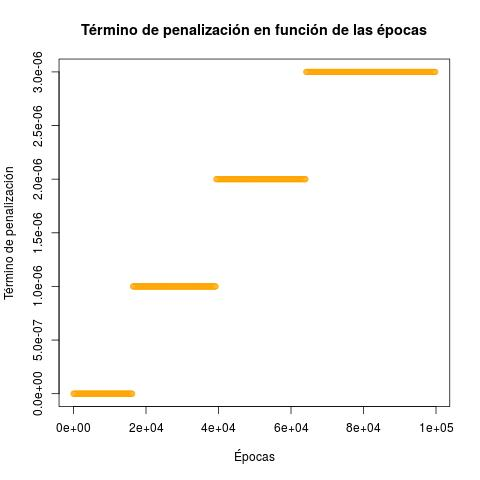
\includegraphics[width=\textwidth]{penalizacion1}
        %\label{fig:gull}
        \caption{Valor del término de penalización en función de las épocas}
    \end{subfigure}
    \caption{Resultados del algoritmo de regularización weight-decay utilizando un valor $\gamma = 10^{-8}$. Las curvas azules representan el MSE de entrenamiento y las verdes de test.}
\end{figure}



 \begin{figure}
    \centering

    \begin{subfigure}[b]{0.45\textwidth}
        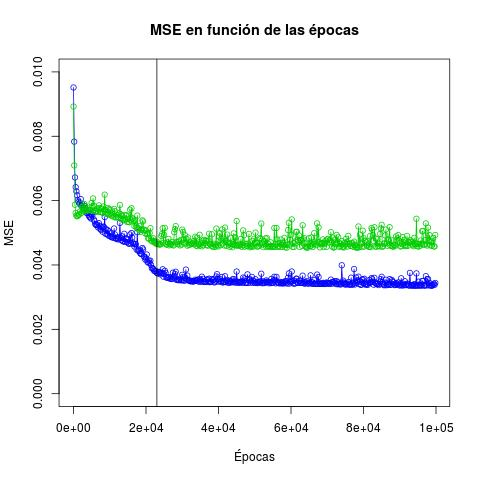
\includegraphics[width=\textwidth]{ejercicioD2}
        %\label{fig:tiger}
		\caption{MSE en test y entrenamiento en función de las épocas. }
    \end{subfigure}
      ~ %add desired spacing between images, e. g. ~, \quad, \qquad, \hfill etc. 
      %(or a blank line to force the subfigure onto a new line)
    \begin{subfigure}[b]{0.45\textwidth}
        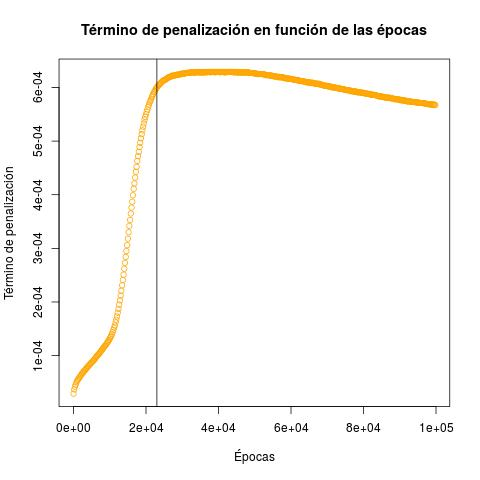
\includegraphics[width=\textwidth]{penalizacion4}
        %\label{fig:gull}
        \caption{Valor del término de penalización en función de las épocas}
    \end{subfigure}
    \caption{Resultados del algoritmo de regularización weight-decay utilizando un valor $\gamma = 10^{-5}$. Las curvas azules representan el MSE de entrenamiento y las verdes de test.}
\end{figure}



\section*{Ejecicio E}
En este ejercicio se pide entrenar redes neuronales para los conjuntos de datos de las gausianas diagonales y paralelas, aumentando la dimensión de éstas. 

\bigskip

En la Figura 16 se presentan las gráficas de error porcentual en test en función de las dimensiones utilizadas, para el algoritmo c4.5 de árboles de decisión y backpropagation de redes neuronales.

\begin{figure}
    \centering
	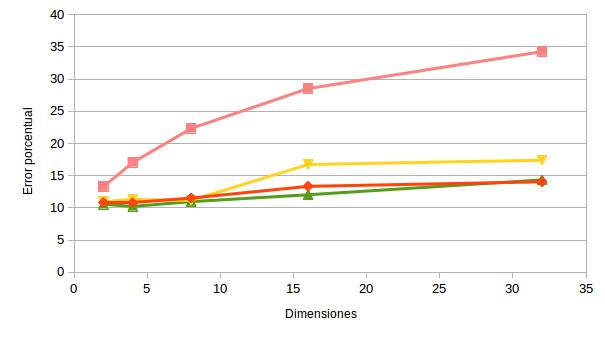
\includegraphics[scale=0.7]{ejercicioE}
	\caption{Curvas de error porcentual en test en función de las dimensiones, para las gausianas diagonales y paralelas. Las curvas rosa y naranja son las obtenidas con el algoritmo c4.5 para las gausianas diagonales y paralelas, respectivamente. Las curvas amarilla y verde se obtuvieron con el algoritmo backpropagation para las gausianas diagonales y paralelas, respectivamente. }
\end{figure} 

\bigskip

Primero analizaremos la gráfica para las gausianas paralelas. De lo observado en dicha figura, se puede suponer que las curvas naranja y verde corresponden a la misma curva de error.\\
En la Figura 17 se muestran las gráficas de las predicciones para backpropagation y c4.5 para 4 y 8 dimensines. Naturalmente, dado que no se pueden graficar tantas dimensiones, se optó por hacer gráficas en donde se comparan todas las variables de a dos. De esta manera, se pueden apreciar las relaciones entre éstas. En ambos casos se puede ver que al dividir la clase con la primera dimensión, las gausianas se dividen correctamente. Por el contrario, al graficar otras combinaciones de variables, las clases se ven mezcladas. De esto se puede deducir que ambos algoritmos están haciendo predicciones muy similares y correctas, ya que en las gausianas paralelas la única dimensión que debe ser tenida en cuenta para hacer la clasificación indicada, es la primera.   


\begin{figure}
    \centering

~ %add desired spacing between images, e. g. ~, \quad, \qquad, \hfill etc.
    \begin{subfigure}[b]{0.45\textwidth}
        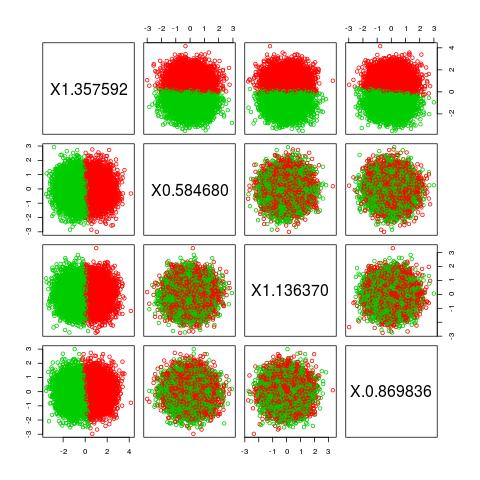
\includegraphics[width=\textwidth]{prediccionB4}
        \caption{Resultados utilizando backpropagation para 4 dimensiones}  
        %\label{fig:tiger}
    \end{subfigure}
      ~ %add desired spacing between images, e. g. ~, \quad, \qquad, \hfill etc. 
      %(or a blank line to force the subfigure onto a new line)
    \begin{subfigure}[b]{0.45\textwidth}
        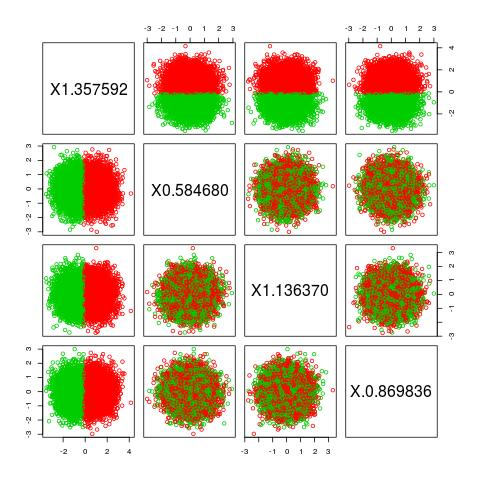
\includegraphics[width=\textwidth]{prediccionB4tree}
        \caption{Resultados utilizando c4.5 para 4 dimensiones}  
        %\label{fig:gull}
    \end{subfigure}


~ %add desired spacing between images, e. g. ~, \quad, \qquad, \hfill etc.
    \begin{subfigure}[b]{0.45\textwidth}
        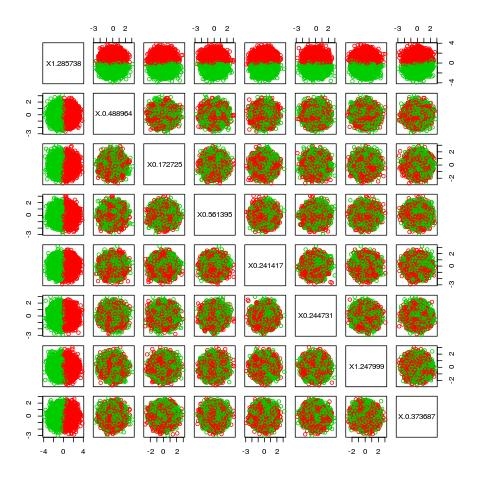
\includegraphics[width=\textwidth]{prediccionB8}
        \caption{Resultados utilizando backpropagation para 8 dimensiones}  
        %\label{fig:tiger}
    \end{subfigure}
      ~ %add desired spacing between images, e. g. ~, \quad, \qquad, \hfill etc. 
      %(or a blank line to force the subfigure onto a new line)
    \begin{subfigure}[b]{0.45\textwidth}
        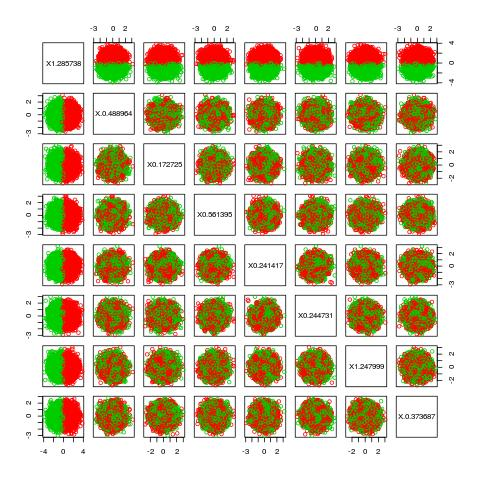
\includegraphics[width=\textwidth]{prediccionB8tree}
        \caption{Resultados utilizando c4.5 para 8 dimensiones}  
        %\label{fig:gull}
    \end{subfigure}

   \caption{Gráficas de las predicciones para las gausianas paralelas de 4 y 8 dimensiones para backpropagation y c4.5.}
\end{figure}

\bigskip

Al observar las curvas de error para las gausianas diagonales tanto para c4.5 como para backpropagation (rosa y amarilla, respectivamente), se nota que se está en un caso muy distinto al anterior, ya que ambas curvas presentan distintas tendencias. Si bien las dos son crecientes, la curva de error para c4.5 crece considerablemente más rápido que la curva de error para backpropagation.  \\
La Figura 18 es análoga a la Figura 17, pero considerando el caso de las gausianas diagonales. Allí se puede observar que las predicciones para los distintos algoritmos difieren, siendo mejor la correspondiente a backpropagation. Justamente, en cada gráfica de combinación de variables, dicho algoritmo hace una división por clases con una tendencia diagonal. Por el contrario, en el caso de las predicciones obtenidas con c4.5, se observa que la división por clases es confusa. Incluso en algunos casos parecieran verse las terminaciones \textquotedblleft escalonadas\textquotedblright que se discutieron en el práctico anterior.\\
A su vez, si se compara la Figura 18 (a) con la Figura 18 (c), se puede observar que la división diagonal de las clases empeora con el aumento en el número de dimensiones. Naturalmente, esto se corresponde con el aumento del error que se aprecia en la Figura 16.

\bigskip

Considerando que el caso de las gausianas paralelas y diagonales es el mismo problema pero teniendo los datos distribuídos de manera diferente con respecto a los ejes,
una conclusión de este ejercicio, teniendo también en cuenta lo analizado en el práctico anterior, debe ser la importancia de la ubicación de los datos en el plano.\\
A su vez, también se debe reparar en cómo el aumento de dimensiones eleva el error, aún cuando se trata del mismo problema, pero en más dimensiones.

\begin{figure}
    \centering

~ %add desired spacing between images, e. g. ~, \quad, \qquad, \hfill etc.
    \begin{subfigure}[b]{0.45\textwidth}
        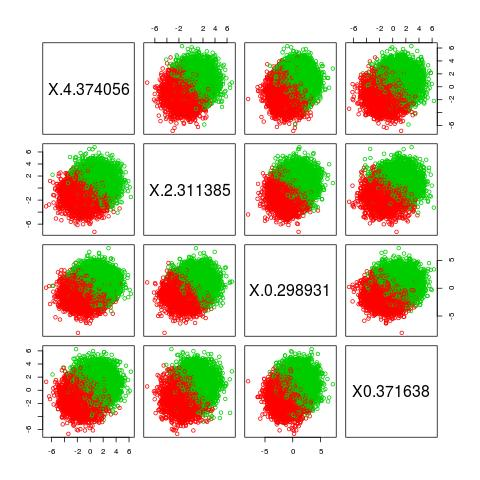
\includegraphics[width=\textwidth]{prediccionA4}
        \caption{Resultados utilizando backpropagation para 4 dimensiones}  
        %\label{fig:tiger}
    \end{subfigure}
      ~ %add desired spacing between images, e. g. ~, \quad, \qquad, \hfill etc. 
      %(or a blank line to force the subfigure onto a new line)
    \begin{subfigure}[b]{0.45\textwidth}
        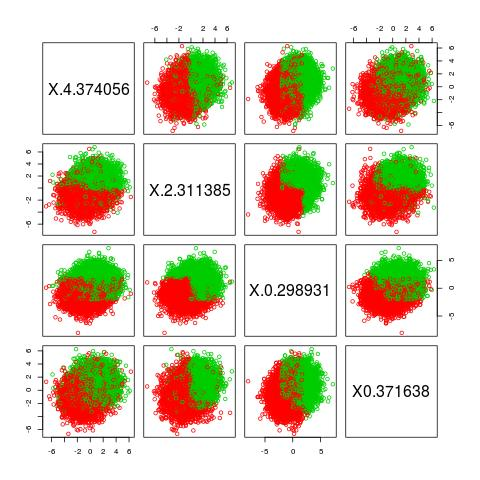
\includegraphics[width=\textwidth]{prediccionA4tree}
        \caption{Resultados utilizando c4.5 para 4 dimensiones}  
        %\label{fig:gull}
    \end{subfigure}


~ %add desired spacing between images, e. g. ~, \quad, \qquad, \hfill etc.
    \begin{subfigure}[b]{0.45\textwidth}
        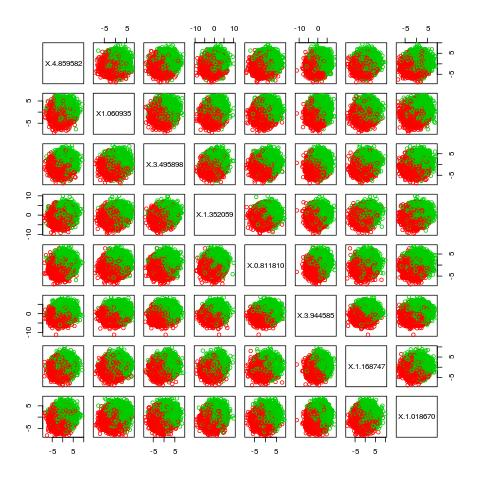
\includegraphics[width=\textwidth]{prediccionA8}
        \caption{Resultados utilizando backpropagation para 8 dimensiones}  
        %\label{fig:tiger}
    \end{subfigure}
      ~ %add desired spacing between images, e. g. ~, \quad, \qquad, \hfill etc. 
      %(or a blank line to force the subfigure onto a new line)
    \begin{subfigure}[b]{0.45\textwidth}
        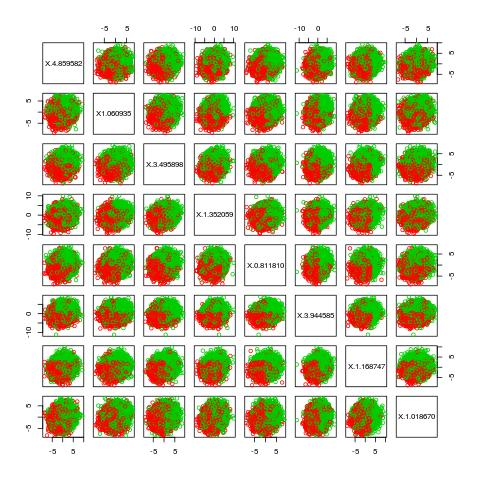
\includegraphics[width=\textwidth]{prediccionA8tree}
        \caption{Resultados utilizando c4.5 para 8 dimensiones}  
        %\label{fig:gull}
    \end{subfigure}

   \caption{Gráficas de las predicciones para las gausianas diagonales de 4 y 8 dimensiones para backpropagation y c4.5.}
\end{figure}


\section*{Ejercicio F}

En este ejercicio se pide modificar el código que implementa el algoritmo backpropagation para que pueda resolver problemas de clasificación en los cuales existen más de dos clases, y probar dicha modificación para los conjuntos de datos \textit{iris} y \textit{faces}.  

\bigskip

En este caso, se optó por continuar con arquitecturas de redes neuronales en donde existe una sola neurona de salida, ya que es la forma más inmediata de extender el programa. De esta forma, el algoritmo siempre considera que las clases son números naturales crecientes consecutivos, empezando por el cero. Es decir, si se indica que la cantidad de clases es 3, entonces el algoritmo considera que las clases son 0,1 y 2.\\
Por lo tanto, la primera modificación realizada es que los archivos de configuración deben indicar cuántas clases existen en el problema de clasificación. \\
Por otro lado, se modificó la función \textit{propagar}, para que calculara el porcentaje de puntos mal clasificados, para la cantidad de clases existentes. En la versión dada en el enunciado, el problema estaba resuelto únicamente para dos clases.\\
A su vez, se creó una función \textit{propagar2}, idéntica a \textit{propagar}, exceptuando que genera un archivo \textit{predicciones\_discretas}. Este archivo es equivalente al generado al ejecutar el código del archivo \textit{discretiza}, dado en el enunciado del trabajo. La función \textit{propagar2} es llamada una única vez en la ejecución del algoritmo, para guardar las predicciones discretas finales para el conjunto de test. Esto se realizó para verificar cómo clasifica la nueva versión del algoritmo.

\bigskip
Una clara contra de esta extensión es que los valores objetivos no estarán entre 0 y 1 o valores similares. Por el contrario, mientras más clases existan, las salidas deseadas llegarán a valores mayores. 

\bigskip
En cuanto a los resultados, para el conjunto de datos iris se utilizaron 4 neuronas intermedias, 10000 iteraciones, learning rate de 0.01 y momentum de 0.5, obteniéndose en la mayor parte de las ejecuciones un error discreto en test de 0\%. En la Figura 19 se grafica el MSE y la cantidad de puntos mal clasificados en función de las épocas. Allí se puede observar que la tendencia de los MSE es disminuír . Sin embargo, si se observa la Figura 19 (b) se puede notar que el error discreto varía entre unos pocos valores, pero la tendencia no es disminuír. En el caso del error discreto en test, el resultado es clasificar correctamente todos los puntos, o errarle a uno de ellos. El problema es que esto no pareciera mejorar con la cantidad de iteraciones. Sin embargo, se puede decir que se logra un buen resultado para este problema.

\begin{figure}
    \centering

~ %add desired spacing between images, e. g. ~, \quad, \qquad, \hfill etc.
    \begin{subfigure}[b]{0.45\textwidth}
        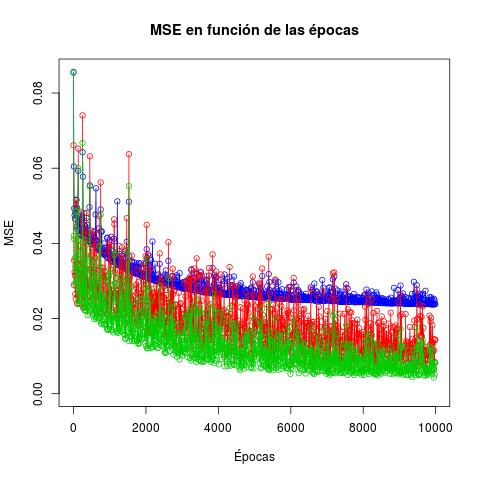
\includegraphics[width=\textwidth]{iris2}
        \caption{MSE en función de las épocas.}  
        %\label{fig:tiger}
    \end{subfigure}
      ~ %add desired spacing between images, e. g. ~, \quad, \qquad, \hfill etc. 
      %(or a blank line to force the subfigure onto a new line)
    \begin{subfigure}[b]{0.45\textwidth}
        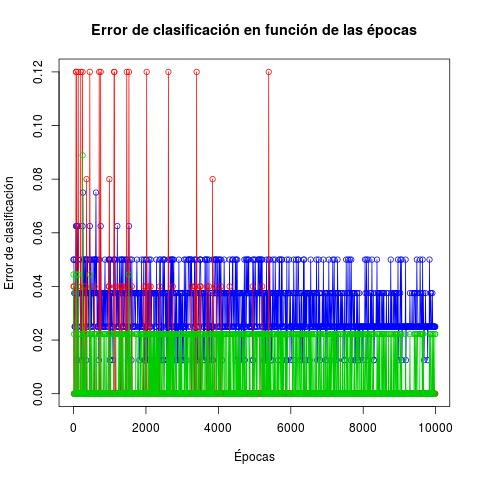
\includegraphics[width=\textwidth]{iris2Porcentual}
        \caption{Cantidad de puntos mal clasificados en función de las épocas}  
        %\label{fig:gull}
    \end{subfigure}

   \caption{Gráficas de los resultados para el conjunto de datos iris. Las curvas azules corresponden a entrenamiento, las verdes a test y las rojas a validación.}
\end{figure}

\bigskip
Por el contrario, para el conjunto de datos faces, el resultado que se obtiene con este método es de un acierto del 25\%, equivalente a asignar clases al azar (es decir, el peor resultado posible). Esto ocurre porque el algoritmo clasifica a todos los puntos como si fueran de la clase 1. \\
Por otro lado, el algoritmo utilizado por el autor del libro, logra un acierto del 90\%. La principal diferencia que observo entre la propuesta de Mitchell y la realizada en este trabajo es la forma en que se codifica la salida. En el libro se propone una codificacion \textit{1-de-n}. Es decir, en lugar de utilizar una única neurona de salida, utiliza 4, cada una de ellas representando una de las clases. La neurona con el valor más alto, indica la predicción de la red neuronal. Esto le  provee mayor grado de libertad para representar la función objetivo. A su vez, la diferencia entre el valor más alto y el segundo más alto puede ser usado como una medida de confianza de la predicción.\\
Otra diferencia de importancia entre ambos algoritmos, es que en el libro no se representa ninguna clase con valor 0 o 1, si no que se elige 0.9 como el valor que indica la clase correspondiente y 0.1 para las demás salidas. Esto se diseña así ya que no se puede producir la salida 0 o 1 para una cantidad de pesos finita, y esto fuerza a los pesos a crecer demasiado. 

\bigskip
Como conclusión de este ejercicio, se puede decir que, por un lado, posiblemente para prroblemas de clasificación de más de dos clases sea más propicio utilizar una codificación de la salida \textit{1-de-n}, frente a una única neurona de output. A su vez, es importante tener en cuenta los valores que toman las clases. Es preferible que sean valores perteneceientes al rango (0,1).

\end{document}


